\documentclass[main.tex]{subfiles}
\usepackage[table,xcdraw]{xcolor}
\usepackage{bm}
\usepackage{wallpaper}
\usepackage{booktabs}
\usepackage{array}
\usepackage{ctex}
\usepackage{longtable}
\usepackage{physics}
\usepackage{fancyhdr}
\usepackage{graphicx} % Required for inserting images
\usepackage{float} %指定图片位置
\usepackage{caption}
\usepackage{pdfpages}
\usepackage{color}
\usepackage{rotating}
\usepackage{tabularray}
\usepackage{xeCJK}
\usepackage{verbatim}
\usepackage{type1cm}
\usepackage{tocloft}
\usepackage{multicol}
\usepackage{amssymb}
\usepackage{amsmath}
\usepackage{float}
\usepackage{wrapfig}
\usepackage{diagbox}
\usepackage{multirow}
\usepackage{subfigure}
\usepackage{svg}
\usepackage[hidelinks]{hyperref}
\usepackage[a4paper,left=2.85cm,right=2.85cm,top=2.54cm,bottom=2.54cm]{geometry}
\renewcommand{\normalsize}{\fontsize{14}{16}\selectfont}


\begin{document}
\chapter{静磁场}
\section{矢势}
\subsection{矢势的引入与库伦规范}
由静磁场中的Maxwell方程组\ref{Maxwell}
\begin{align}
    &\nabla \cdot \boldsymbol{B} = 0\\
    \label{er}&\nabla \times \boldsymbol{B} = \mu _0 \boldsymbol{J}
\end{align}

我们肯定能找到一个矢量场$A$满足$\boldsymbol{B} = \nabla \times \boldsymbol{A}$.\ $\boldsymbol{A}$称为磁场的\textbf{矢势}.把$\boldsymbol{B}$对任一以$L$为边界的曲面$S$积分得到:
\begin{align}
    \int_{S}^{} \boldsymbol{B} \cdot \mathrm{d} \boldsymbol{S} = \int_{S}^{} \nabla \times \boldsymbol{A} \cdot \mathrm{d} \boldsymbol{S} = \oint_{L}^{} \boldsymbol{A} \cdot \mathrm{d} \boldsymbol{l} 
\end{align}

由$\nabla \times \nabla \varphi = 0$,我们可以得到磁场矢势的性质:
\begin{align}
    &\nabla \times (\boldsymbol{A} + \nabla \varphi) = \nabla \times \boldsymbol{A}\\
    &\boldsymbol{A} + \nabla \varphi = \boldsymbol{A}
\end{align}

由于这种任意性,我们需要对其加上限制条件使得$\boldsymbol{A}$对$\boldsymbol{B}$唯一确定:
\begin{align}
    \nabla \cdot \boldsymbol{A} = 0
\end{align}

称之为\textbf{Coulomb规范}.

\subsection{矢势微分方程}
将$\boldsymbol{B} = \nabla \times \boldsymbol{A}$代入式\ref{er}中得到:
\begin{align}
    \nabla \times (\nabla \times \boldsymbol{A}) = \mu _0 \boldsymbol{J}
\end{align}

利用矢量分析公式\ref{nabla7}有
\begin{align}
    \nabla \times (\nabla \imes \boldsymbol{A}) = \nabla(\nabla \cdot \boldsymbol{A}) - \nabla ^2 \boldsymbol{A}
\end{align}

代入Coulomb规范条件$\nabla \cdot \boldsymbol{A} = 0$,得到矢势$\boldsymbol{A}$的微分方程
\begin{align}
    &\nabla ^2 \boldsymbol{A} = -\mu _0 \boldsymbol{J}\\
    &(\nabla \cdot \boldsymbol{A} = 0)
\end{align}

或替换成标量的Poisson方程:
\begin{align}
    \label{poisson2}\nabla ^2 A_i = -\mu _0 J_i\ \ (i = 1,2,3)
\end{align}

在之前讨论电势问题时,同样有Poisson方程$\nabla ^2\varphi = -\frac{\rho}{\varepsilon _0}$,其解为$\varphi = \frac{1}{4\pi \varepsilon _0}\int \frac{\rho(\boldsymbol{x}'\mathrm{d}V')}{r}$.仿照此结果我们可以写出\ref{poisson2}的解:
\begin{align}
    \boldsymbol{A}(\boldsymbol{x}) = \frac{\mu}{4\pi}\int _{V}^{}\frac{\boldsymbol{J}(\boldsymbol{x}')\mathrm{d}V'}{r}
\end{align}

\begin{wrapfigure}{r}{4cm}
	\centering
	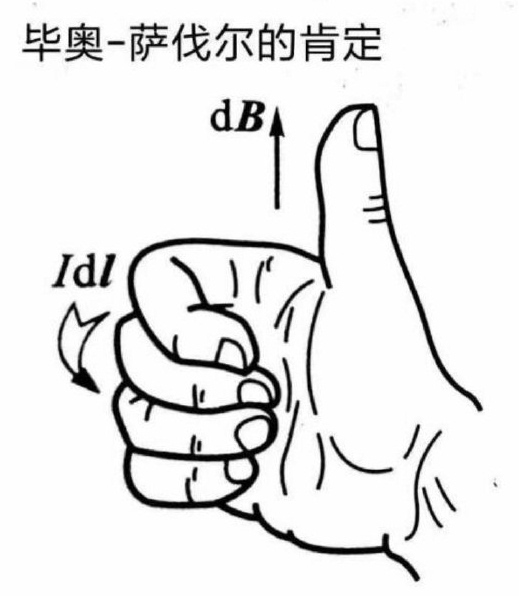
\includegraphics[width=0.9\linewidth]{Biot-Savart.jpg}
\end{wrapfigure}

对其取旋度即可得到$\boldsymbol{B}$
\begin{align}
    \boldsymbol{B} = \nabla \times \boldsymbol{A} = \frac{\mu}{4\pi}\int _{V}^{}\frac{\boldsymbol{J}\times \boldsymbol{r}}{r^3}\mathrm{d}V'
\end{align}

由代换$\boldsymbol{J}\mathrm{d}V'\to \boldsymbol{J}\mathrm{d}\boldsymbol{l}$可以推导出\textbf{Biot-Savart定律}
\begin{align}
    \boldsymbol{B} =  \frac{\mu}{4\pi}\oint_{L}^{} \frac{\boldsymbol{J}\mathrm{d}\boldsymbol{l} \times \boldsymbol{r}}{r^3}
\end{align}

对于矢势$\boldsymbol{A}$,如果取Coulomb规范条件,则可以证明在两介质分界面上矢势连续.
\begin{align}
    \boldsymbol{A}_2 = \boldsymbol{A}_1
\end{align}

\section{磁标势}
\begin{wrapfigure}{l}{5.5cm}
	\centering
	\includesvg[width=0.9\linewidth]{cibiaoshi.svg}
\end{wrapfigure}

\textbf{必要条件:}

由环路定理可得:
\begin{align}
    \oint_{L} \boldsymbol{H} \cdot \mathrm{d}\boldsymbol{l} = \int _{S} \boldsymbol{J} \cdot \mathrm{d} \boldsymbol{S}
\end{align}

当所围成环路内不含电流,则
\begin{align}
    \oint_{L} \boldsymbol{H} \cdot \mathrm{d}\boldsymbol{l} = \int _{S} \boldsymbol{J} \cdot \mathrm{d} \boldsymbol{S} =0
\end{align}

此时可以类比电势引入磁标势$\phi$描述磁场.定义
\begin{align}
    &\boldsymbol{H} = -\nabla \phi\\
    &\nabla ^2 \phi = -\frac{\rho_m}{\mu _0}
\end{align}

无磁荷时,Poisson方程变为Laplace方程$\nabla ^2\phi = 0$,可以仿照对电势的处理写出其通解\ref{Laplacejie}.

\section{磁多极矩}
\subsection{矢势的多极展开}
类比之前对电势的泰勒展开,同样可以把磁场矢势展开为
\begin{align}
    &\boldsymbol{A}(\boldsymbol{x}) = \frac{\mu _0}{4\pi}\int _{V}\boldsymbol{J}'(\boldsymbol{x})\left[\frac{1}{R} - \boldsymbol{x}'\cdot \nabla \frac{1}{R}+\frac{1}{2!} \sum_{i,j}x_i' x_j' \frac{\partial ^2}{\partial x_i \partial x_j} \frac{1}{R} \right] \mathrm{d}V'
\end{align}

其中展开式第一项
\begin{align}
    \boldsymbol{A}^{(0)} = \frac{\mu _0}{4\pi R}\int _{V}\boldsymbol{J}'(\boldsymbol{x})\mathrm{d}V' = \frac{\mu _0}{4\pi R}I\int _{V}\mathrm{d}\boldsymbol{l} = 0
\end{align}

即展开式不含磁单极项.第二项
\begin{align}
    \boldsymbol{A}^{(1)} &= -\frac{\mu _0}{4\pi}\int _{V} \boldsymbol{J}(\boldsymbol{x}')\boldsymbol{x}'\cdot \nabla \frac{1}{R}\mathrm{d}V'\\
    & = \frac{\mu _0}{4\pi R^3}\cdot \frac{I}{2}\oint _{L}(\boldsymbol{x}' \times \mathrm{d} \boldsymbol{l}')\times \boldsymbol{R}\\
    & = \frac{\mu _0}{4\pi}\  \frac{\boldsymbol{m} \times \boldsymbol{R}}{R^3}
\end{align}

式中
\begin{align}
    \boldsymbol{m} = \frac{I}{2} \oint_{L} \boldsymbol{x}' \times \mathrm{d} \boldsymbol{l}' = \frac{1}{2} \int_{V} \boldsymbol{x}' \times \boldsymbol{J}(\boldsymbol{x}') \mathrm{d} \boldsymbol{V}' 
\end{align}

为电流圈的磁矩.

\subsection{磁场的能量}

由\ref{nengliang}得到,静磁场能量
\begin{align}
    W& = \frac{1}{2}\int_{V}\boldsymbol{B}\cdot \boldsymbol{H} \mathrm{d}V\\
    & = \frac{1}{2}\int_{V} (\nabla \times \boldsymbol{A}) \cdot \boldsymbol{H} \mathrm{d}V\\
    & = \frac{1}{2}\int_{V}\boldsymbol{A}\cdot \boldsymbol{J} \mathrm{d}V
\end{align}

\section{Aharonov–Bohm效应}
在经典电动力学中,磁场矢势$\boldsymbol{A}$和电势$\varphi$不是有直接观测意义的物理量.\ 但在量子力学中,势$\boldsymbol{A}$和$\varphi$具有可观测的物理效应,这一效应称为\textbf{Aharonov–Bohm效应},简称\textbf{A-B效应}.

\end{document}